\startchapter{Automated Trojan Detection}
\label{chapter:trojanDetection}
\section{Methodology}
Figure~\ref{fig:Concept} provides a visual representation of the basic concept assumed for the purposes of this work. 
All stages of production of an \acrshort{FPGA} implementation are done "in-house" with the exception of the fabrication process. 
It is assumed that any trojan discovered is inserted in the fabrication phase; all other stages are trusted.  
The method of automated trojan detection described in this work would take place in the 'testing' phase of the life-cycle. 
\begin{figure}[h]
	\centering
	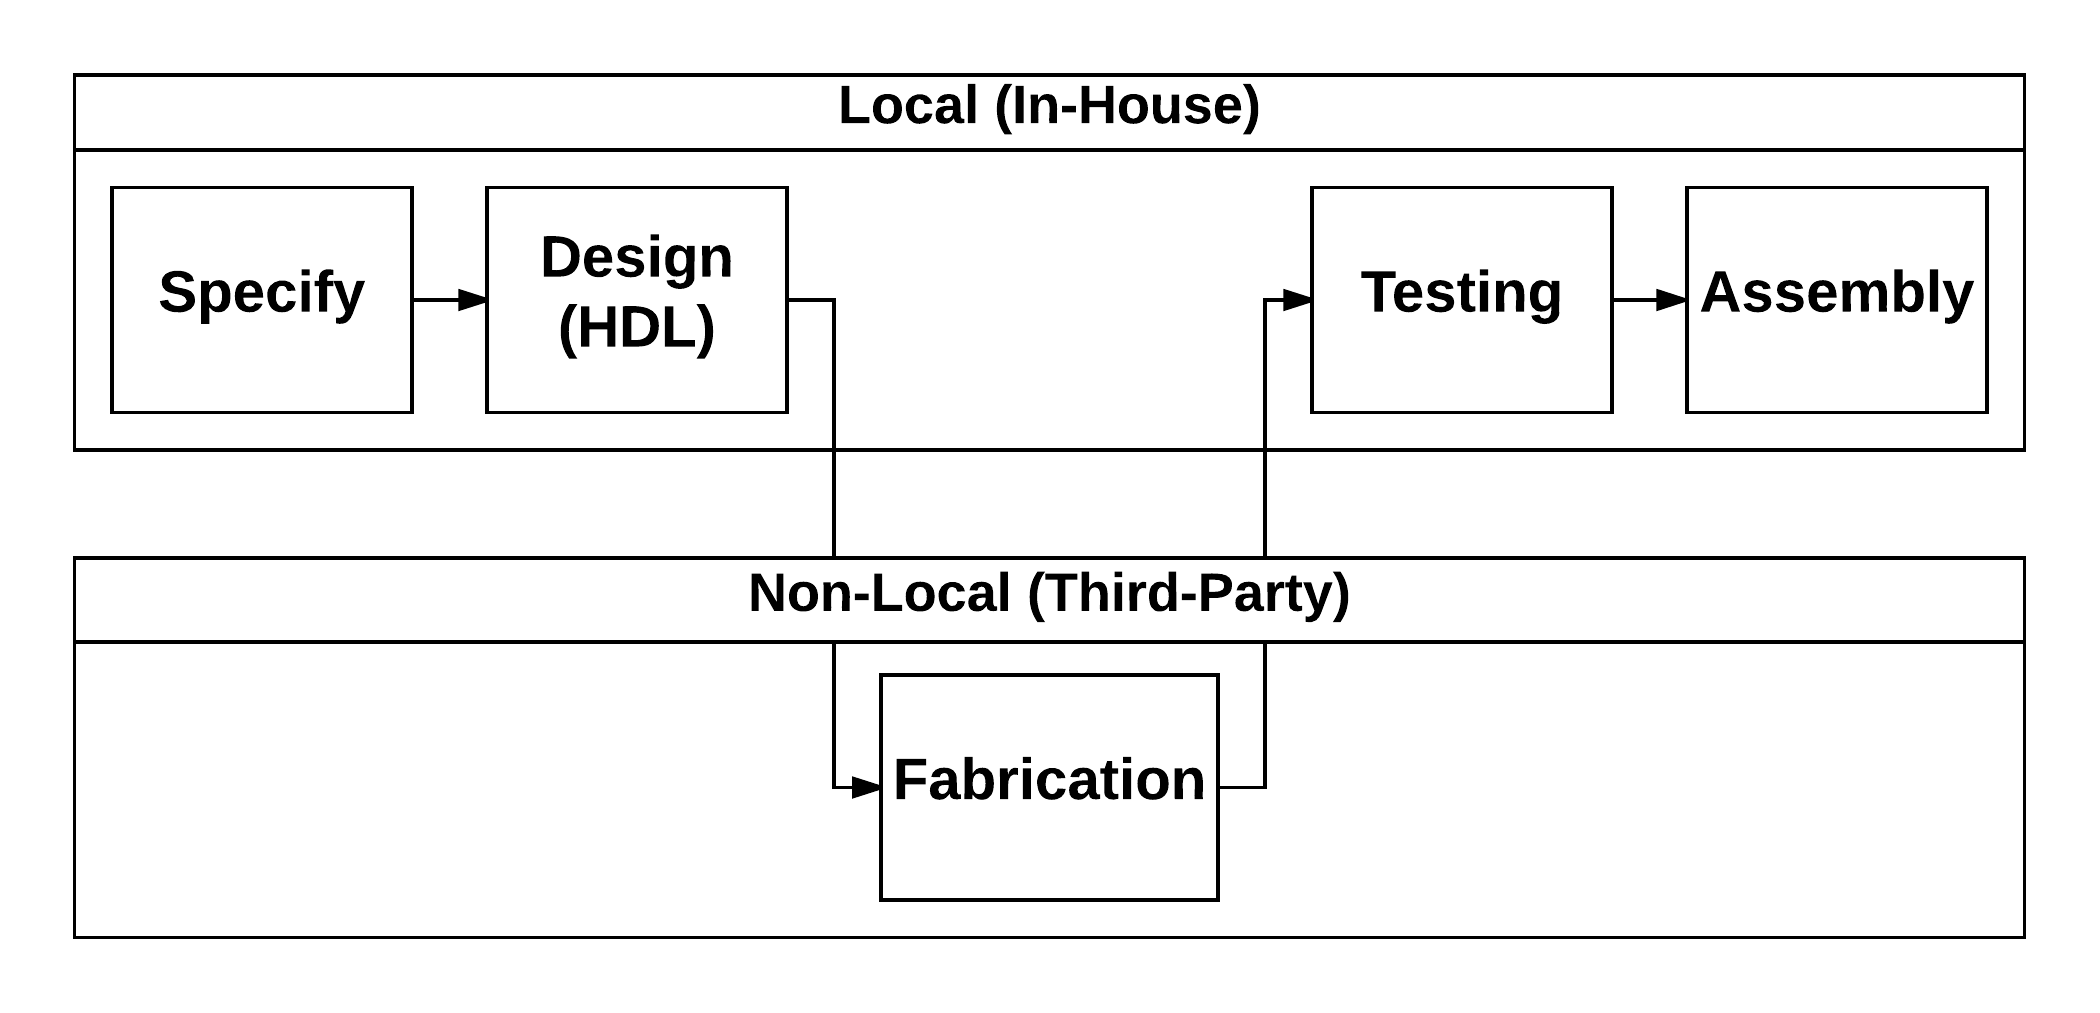
\includegraphics[width=1\linewidth]{figures/Concept}
	\caption[FPGA Life-Cycle]{FPGA Life-Cycle}
	\label{fig:Concept}
\end{figure}

Figure~\ref{fig:methodologyOverview} shows an overview of the trojan detection scheme.
\acrshort{FPGA} designs are written in a \acrfull{HDL}.
\Xilinx provides a series of \acrfull{UI} or command line tools to process the design known as the 'tool-chain'.
The tool chain generates a series of files that are used for a variety of purposes.
The Bit file is a binary representation of the design to be implemented.
It is referred to as the \gls{Bitstream} or Configuration \gls{Bitstream} and is the final form which is loaded into the device.
\begin{figure}
	\centering
	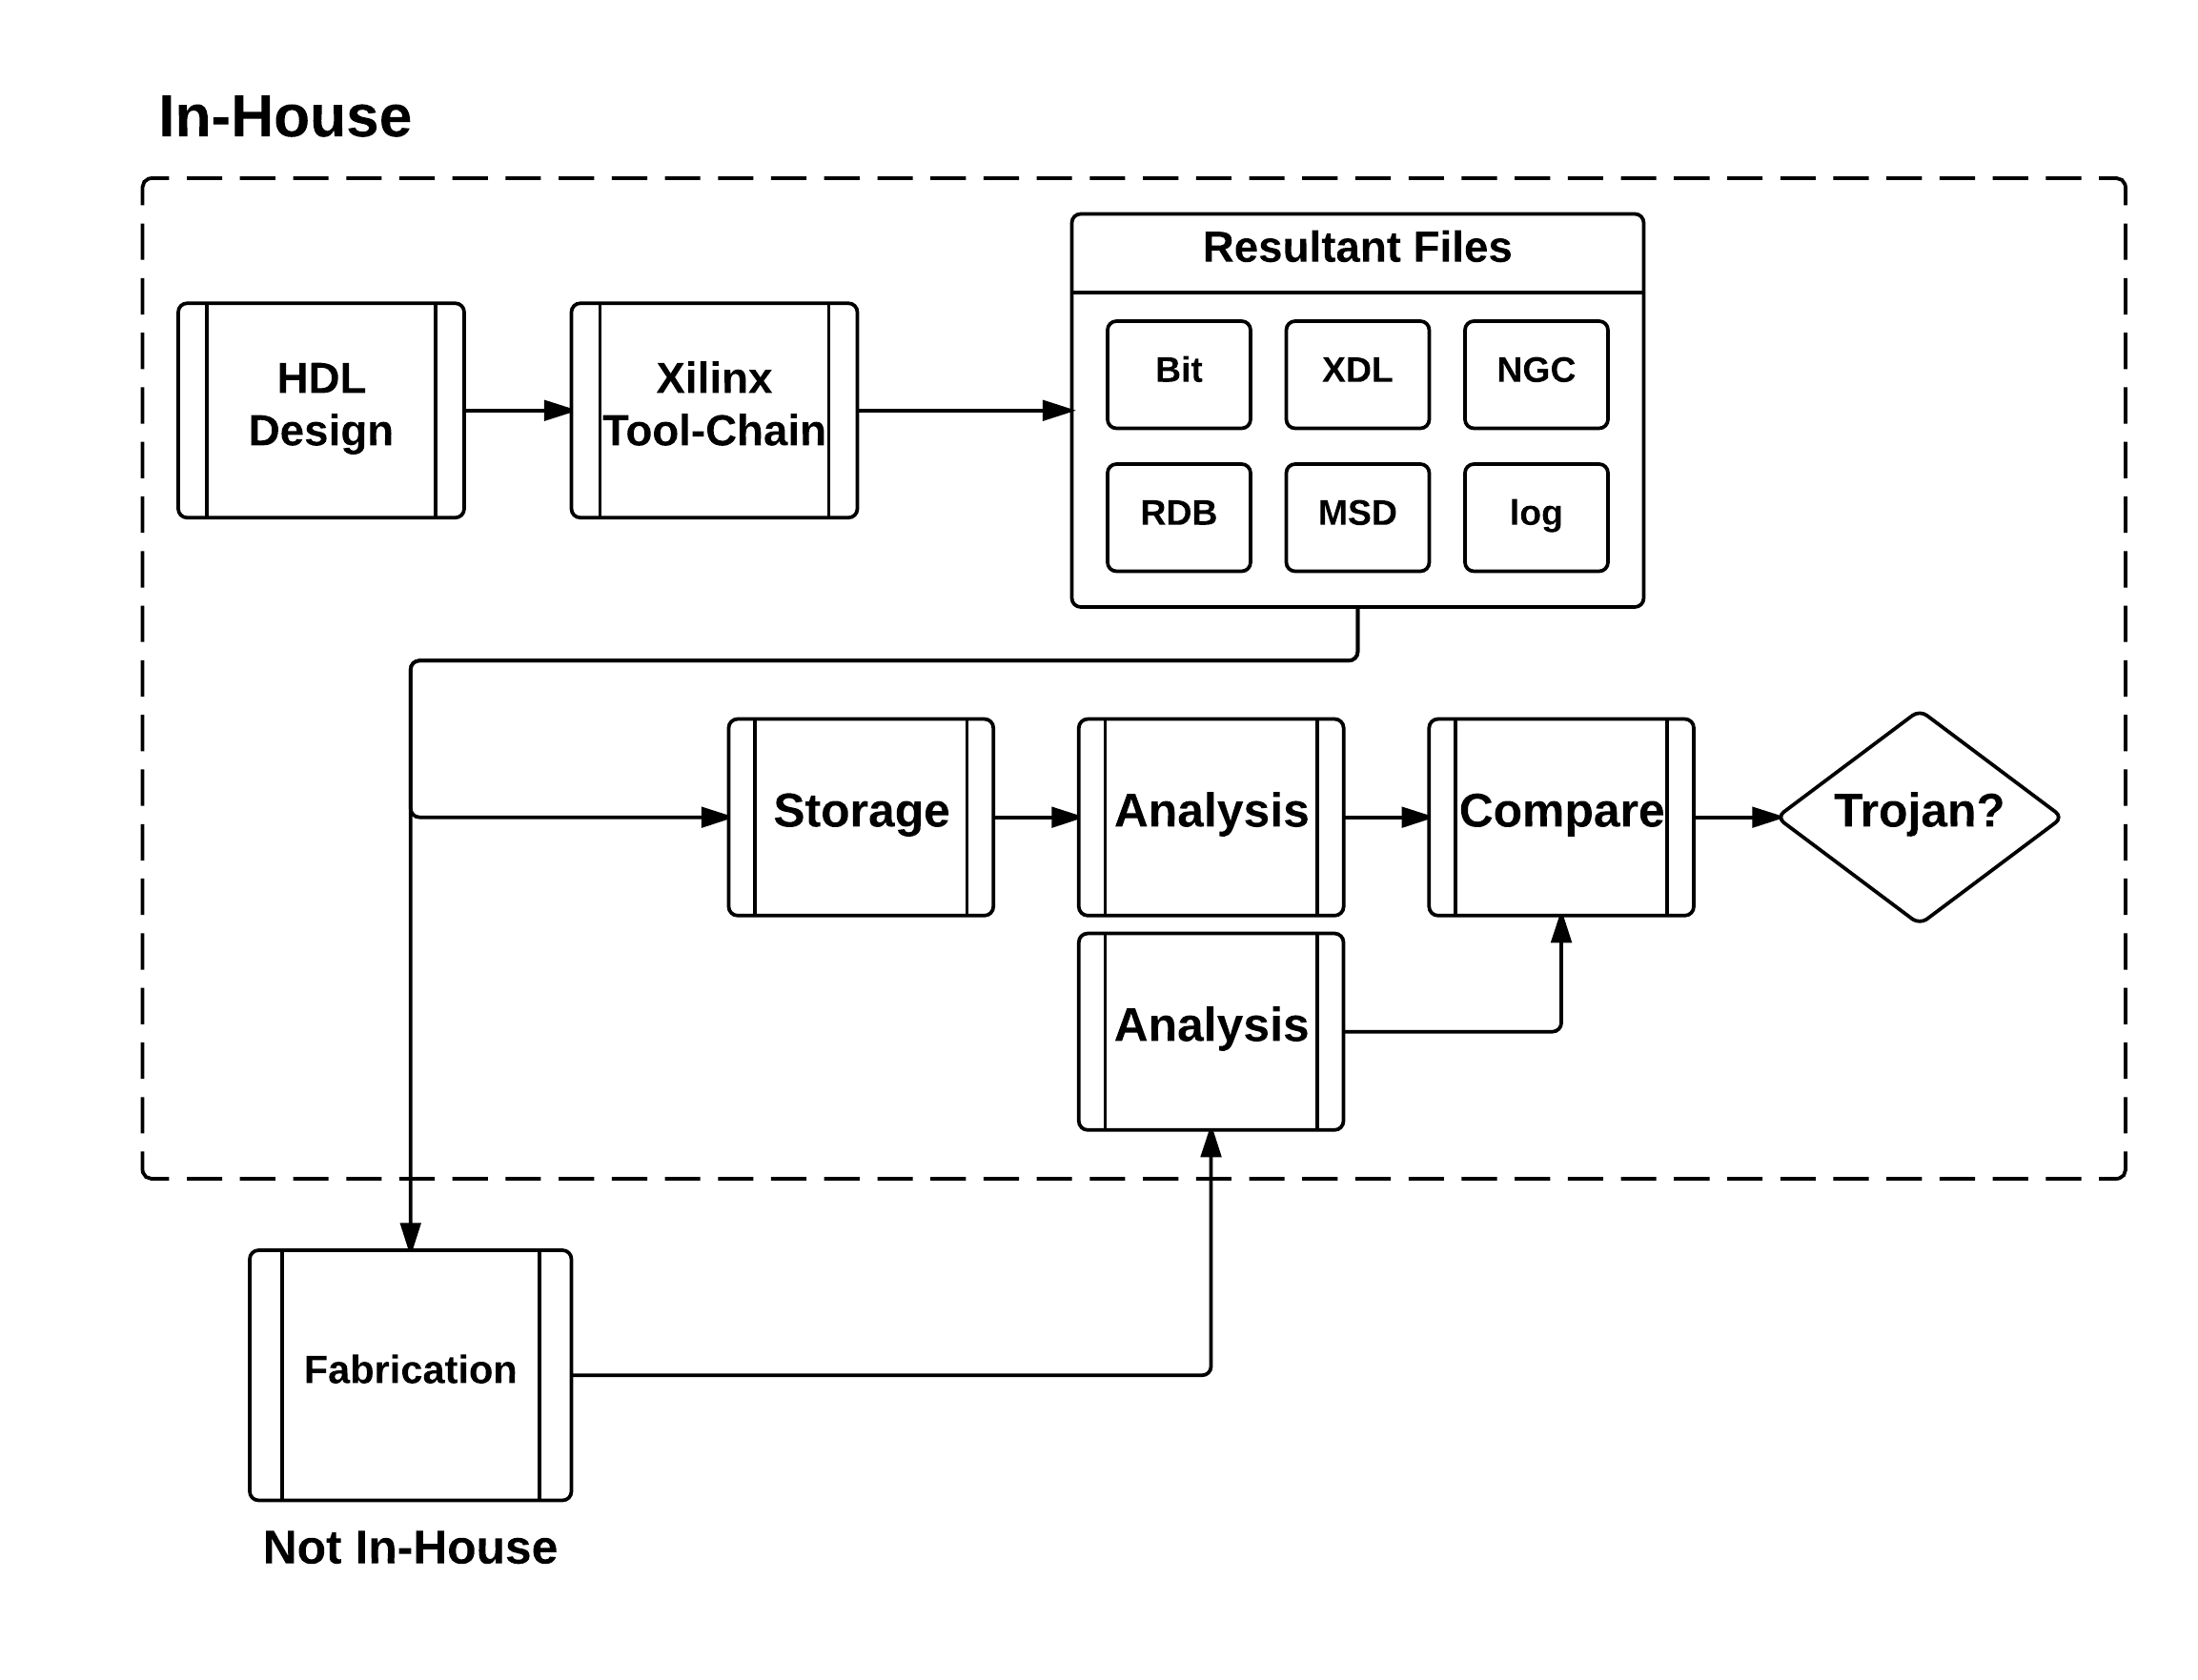
\includegraphics[width=1\linewidth]{Figures/methodologyOverview}
	\caption[Methodology Overview]{Methodology Overview}
	\label{fig:methodologyOverview}
\end{figure}
This Bit file is also one of the primary files sent to the fabrication house where it will be implemented onto the batch of devices ordered.
The resultant files are kept in secure storage while a copy is sent to be fabricated; these 'clean' copies are reffered to as \gls{golden}.
Though it is known that fabrication houses will often attempt to make optimizations on designs this methodology requires that no such efforts are made.
When the completed batch of fabricated chips are returned the \gls{Bitstream} is extracted via the method described in section~\ref{sec:bitstreamExtraction}. 
That which is extracted is referred to as the \gls{target} \gls{Bitstream}.
The \gls{golden} and \gls{target} \gls{Bitstream}s are analyzed in conjunction to detect differences, described in section~\ref{sec:frameComparison}.
Any discovered differences are then attributed to the corresponding component in the architecture, described in section~\ref{sec:tileMapping}.
Finally, descriptive attributes presented in section~\ref{sec:topology} are returned to the user, described in section~\ref{sec:trojanAttributes}. 

\section{FPGA Architecture and Configuration}
A \Xilinx \acrfull{FPGA} is comprised of a matrix of tiles referred to as the 'gate-array' and is shown in Figure~\ref{fig:FPGA}.
A device can contain anywhere from a couple hundred to a few thousand tiles; they are arranged into columns by type.
An FPGA may have over one-hundred different types of tiles however each column is comprised almost entirely of a single type.
Columns are separated by clock regions as shown by the dashed lines in Figure~\ref{fig:FPGA}.
Each region is an independent array of tiles that uses a dedicated clock resource; this minimizes clock skew from causing undesired timing delays.
\begin{figure}[h]
	\centering
	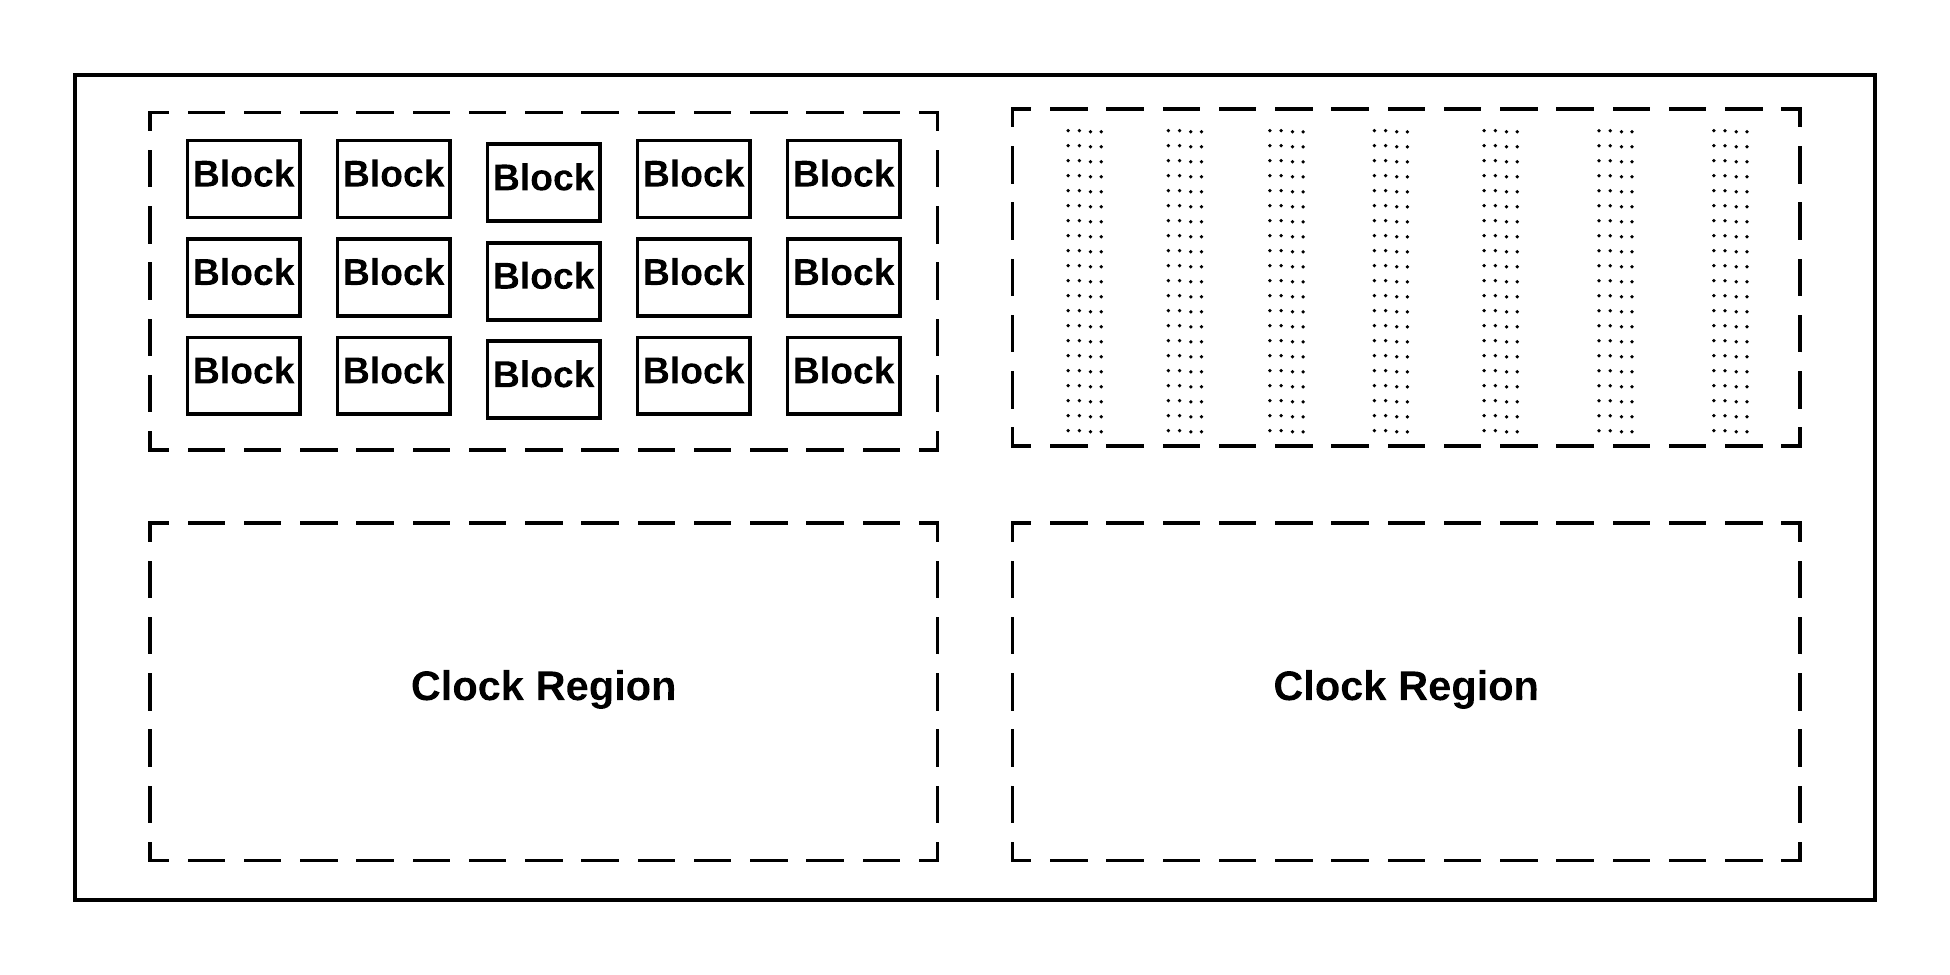
\includegraphics[width=1\linewidth]{figures/FPGA}
	\caption[Rudimentary Layout of a Virtex Gate-Array]{Rudimentary Layout of a Virtex Gate-Array}
	\label{fig:FPGA}
\end{figure}
Though each tile has a designated purposes (ex. \acrfull{IO}, \acrfull{CL}, memory...etc) their functionality can be configured by the user; this is how designs are implemented on a device.
The configuration of each tile is dictated by the \gls{Bitstream}. 
To improve performance the contents of the gate-array is referred to as dynamic.
A dynamic device is unable to retain the contents of its memory when it looses power.
To prevent having to plug in a device and download the configuration every time it is powered on, an external static memory device (i.e. retains its contents with loss of power) holds the \gls{Bitstream}. 
When an \acrshort{FPGA} is powered on the \gls{Bitstream} is loaded from the external memory (often \acrfull{SRAM}) into the gate-array, as can be seen in Figure~\ref{fig:architecture}.

\begin{figure}
\centering
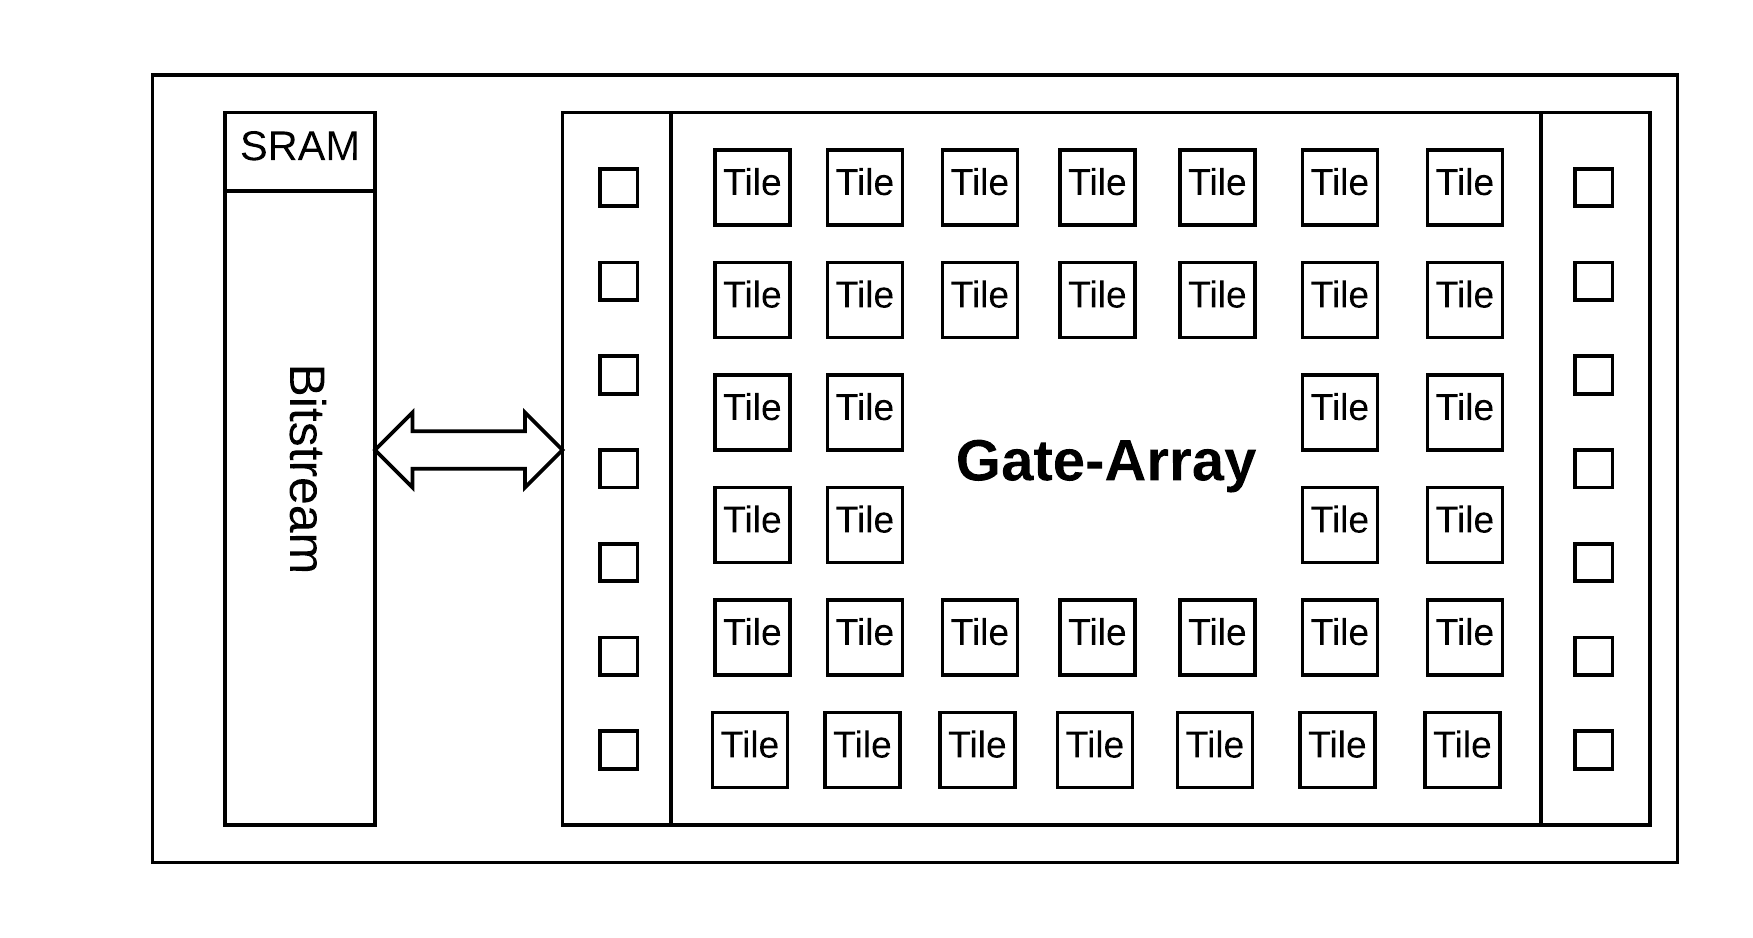
\includegraphics[width=0.9\linewidth]{Figures/architecture}
\caption[FPGA Device Layout]{FPGA Device Layout}
\label{fig:architecture}
\end{figure}

\section{The \acrshort{FPGA} Bitstream} \label{sec:fpgaBitStream}
The \Xilinx bitstream is organized into 'frames'.
A frame is a string of single bits that span from the top to the bottom of a clock region of a device as seen in the top-right quadrant of Figure~\ref{fig:FPGA}.
In other words, each frame affects every tile in a column.
Multiple adjacent frames are required to configure an entire column. 
\section{Bitstream Extraction} \label{sec:bitstreamExtraction}
\section{Frame Comparison} \label{sec:frameComparison}
\section{Tile Mapping} \label{sec:tileMapping}
\section{Trojan Attributes} \label{sec:trojanAttributes}



%This is where you go all out and tell us all about your new discovery and research related to the problem in the previous chapter. No arrogant sweeping statements which cannot be fully justified, but no false modesty either. You must impress your reader that you have accomplished something.
%
%Simply summarized, this chapter should be comprised of at least two main sections, each with appropriate subsections. The first section should describe:
%\begin{itemize}
%\item {what the new approach is;}
%\item {what is really totally new;}
%\item {what is incrementally new;}
%\item {what you built upon.}
%\end{itemize}
%
%The second part should describe fully how the new approach works, both with the overall theoretical exposition (e.g. an algorithm) and with as many examples as necessary for clarity. Remember that if the reader does not understand fully, you will get a lot of questions and doubts. Good examples, good figures, good diagrams with super clear tutorial explanations can be a joy to read and make even a small contribution appear to be more impressive. Are you afraid that if you are too tutorial your work will not seem as deep and difficult? Only shallow people will make such a superficial evaluation, have trust instead in the wisdom of your supervisory committee.
%
%Use at least one good example throughout, and even better if this is one of the examples you used in Chapter 2 to describe the original problem.
%
%By the way, this would be the first chapter I would write. This is what I know best right now, as I just finished working on it. It is clear to me and on the tip of my fingers. Start with your strengths! The second chapter I would write is the next one about the experiments, followed closely by chapter 2 describing the problem. It may not seem intuitive to you, but it works and it is the most productive way I ever found to finish a document.
%
%
%\input chapters/3/sec_latexhelp
